% BEGIN_FOLD (Preamble)
%        File: Masterarbeit.tex
%     Created: Di Mrz 04 02:00  2014 Mitteleuropäische Z
% Last Change: Di Mrz 04 02:00  2014 Mitteleuropäische Z
%
% !TEX TS-program = pdflatex
% !TEX encoding = UTF-8 Unicode

\documentclass[11pt, titlepage=true]{scrreprt} % use larger type; default would be 10pt
\setcounter{secnumdepth}{3} % Überschriften-Nummern bis zur 3. Ebene

\usepackage[utf8]{inputenc} % set input encoding (not needed with XeLaTeX)
\usepackage[ngerman]{babel} 
\usepackage[babel,german=quotes]{csquotes}
\usepackage[T1]{fontenc} % for enabling non-standard characters in
                         % hyphenation-list and smallcaps-boldfont

\usepackage[bibstyle=authortitle, citestyle=authoryear, isbn=false, doi=false,
dashed=false]{biblatex}
\addbibresource{Masterarbeit.bib}

\def^^cc{XXXXX} % Zum Aufspüren von fehlerhaften Zeichen, falls komische Codierungsfehler mit der Bibliographie auftauchen.

% \DeclareUnicodeCharacter{00A0}{~} % for avoiding problems with no-break spaces

%%% PAGE DIMENSIONS
\usepackage{geometry} % to change the page dimensions
\geometry{a4paper} % or letterpaper (US) or a5paper or....
% \geometry{margin=2in} % for example, change the margins to 2 inches all round
% \geometry{landscape} % set up the page for landscape
%   read geometry.pdf for detailed page layout information

\usepackage{graphicx} % support the \includegraphics command and options
\usepackage{tikz} % for graphics produced by R

\graphicspath{{../Abbildungen/}{./Abbildungen/}}

\usepackage[parfill]{parskip} % Activate to begin paragraphs with an empty line rather than an indent
\usepackage{setspace} % Provides the commands \doublespacing, \onehalfspacing,
                      % \singlespacing and \setstretch{baselinestretch} for
                      % controlling the line height

%%% PACKAGES
\usepackage{booktabs} % for much better looking tables
\usepackage[]{longtable}
\usepackage{array} % for better arrays (eg matrices) in maths
%\usepackage{paralist} % very flexible & customisable lists (eg. enumerate/itemize, etc.)
\usepackage{verbatim} % adds environment for commenting out blocks of text & for better verbatim
\usepackage{subfig} % make it possible to include more than one captioned figure/table in a single float
% These packages are all incorporated in the memoir class to one degree or another...
\usepackage{amsmath}
\usepackage{amssymb}
\usepackage{siunitx}
\usepackage{mathtools}
\usepackage{mdframed}
\usepackage{booktabs}
\usepackage{nicefrac}

\usepackage{ifthen}

\usepackage{enumitem} % Aufzaehlungen anpassen (z.B. Buchstaben statt Zahlen))

%%% HEADERS & FOOTERS
\usepackage{fancyhdr} % This should be set AFTER setting up the page geometry
\pagestyle{fancy} % options: empty , plain , fancy
\renewcommand{\headrulewidth}{0pt} % customise the layout...
\lhead{}\chead{}\rhead{}
\lfoot{}\cfoot{\thepage}\rfoot{}
\usepackage{footnote}

%%% SECTION TITLE APPEARANCE
\usepackage{sectsty}
\allsectionsfont{\sffamily\mdseries\upshape} % (See the fntguide.pdf for font help)
% (This matches ConTeXt defaults)

%%% ToC (table of contents) APPEARANCE
\usepackage[nottoc,notlof,notlot]{tocbibind} % Put the bibliography in the ToC
\usepackage[titles,subfigure]{tocloft} % Alter the style of the Table of Contents
\renewcommand{\cftsecfont}{\rmfamily\mdseries\upshape}
\renewcommand{\cftsecpagefont}{\rmfamily\mdseries\upshape} % No bold!

\usepackage[hidelinks]{hyperref}
\usepackage{ragged2e} %für links und rechtsbündige Umgebungen in Tabellen
\usepackage[textsize=tiny, colorinlistoftodos]{todonotes} % TODO-Notizen. Ausschalten mit der Option [disable]
\usepackage[normalem]{ulem} % ermöglicht es, Text mittels \sout und \xout
                            % durchzustreichen

% Überschriften-Stile anpassen
\usepackage{titlesec}
\titleformat{\chapter}[hang]{\sffamily\LARGE\bfseries}{\thechapter\quad}{0pt}{}
\titleformat{\section}[hang]{\sffamily\Large\bfseries}{\thesection\quad}{0pt}{}
\titleformat{\subsection}[hang]{\sffamily\large\bfseries}{\thesubsection\quad}{0pt}{}
\titleformat{\subsubsection}[hang]{\sffamily\large}{\thesubsubsection\quad}{0pt}{}
\titleformat{\paragraph}[hang]{\sffamily\bfseries}{}{}{}
\titlespacing{\chapter}{0pt}{0pt}{12pt}
\titlespacing{\section}{0pt}{12pt}{12pt}
\titlespacing{\paragraph}{0pt}{12pt}{0pt}

%%% Eigene Befehle %%%
\newcommand{\was}[1]{\small\textit{#1}}
\newcommand{\noteS}[1]{\todo[color=blue!40]{\textbf{Sascha: }#1}}
\newcommand{\noteJ}[1]{\todo[color=blue!40]{\textbf{János: }#1}}
\definecolor{prioH}{named}{red}
\definecolor{prioM}{named}{yellow}
\definecolor{prioL}{named}{green}
\newcommand{\textfrac}[2]{\hspace{2pt} \frac{\text{#1}}{\text{#2}}}
\newcommand{\eqnref}[1]{\overset{(\ref{#1})}{=}} % Gleichheitszeichen mit Referenz auf die verwendete Gleichung
\newcommand{\defeq}{\vcentcolon=} %Definitions-Gleichheitszeichen
\newcommand{\eqdef}{=\vcentcolon}
\newcommand{\pfrac}[2]{\frac{\partial #1}{\partial #2}}

% Formeln:
\newcommand{\MIPS}[1][]{
  \ifthenelse {\equal {#1} {}}
  {\text{MIPS}} % if argument is blank
  {\text{MIPS}({#1})} % if an optional argument is given
}
\renewcommand{\P}[1]{P_\text{#1}}
\newcommand{\I}[1]{I_\text{#1}}
\newcommand{\itext}[1]{i_\text{#1}}
\newcommand{\T}[1]{T_\text{#1}}
\newcommand{\n}[1]{n_\text{#1}}
\newcommand{\N}[1]{N_\text{#1}}
\newcommand{\w}[1]{w_\text{#1}}
\renewcommand{\t}[1]{t_\text{#1}}

% Szenarien:
\newcommand{\SzenarioI}{Szenario \textsc{Kleine Wohneinheiten}}
\newcommand{\SzenarioII}{Szenario \textsc{Luhrmannhof}}
\newcommand{\SzenarioIII}{Szenario \textsc{Waschsalon}}

%%% Allgemeine Daten %%%
\newcommand{\autorOne}{Alexander Müller}
\newcommand{\matrikelnrOne}{940597}
\newcommand{\adresseOne}{Gartlager Weg 37, \\49086 Osnabrück}
\newcommand{\telOne}{01578 1901578}
\newcommand{\emailOne}{alemuell@uos.de}

\newcommand{\autorTwo}{János Sebestyén}
\newcommand{\matrikelnrTwo}{939525}
\newcommand{\adresseTwo}{Gartlager Weg 37, \\49086 Osnabrück}
\newcommand{\telTwo}{}
\newcommand{\emailTwo}{jsebesty@uos.de}

%%% Titlepage Expose %%%
\newcommand{\titel}{Ökologische Nachhaltigkeit durch \enquote{Nutzen statt Besitzen}?}
\newcommand{\stitle}{Entwicklung eines Modells zur Ableitung von Kriterien für die Senkung des Umweltverbrauchs durch gemeinschaftliche Produktnutzung}
\newcommand{\art}{Master-Arbeit}
\newcommand{\fachgebiet}{Angewandte Systemwissenschaft}
\newcommand{\betreuungOne}{Katrin Bienge}
\newcommand{\betreuungTwo}{Prof. Dr. Claudia Pahl-Wostl}
\newcommand{\institutOne}{Wuppertal Institut für Klima, Umwelt, Energie}
\newcommand{\institutTwo}{Institut für Umweltsystemforschung, Osnabrück}
\newcommand{\ort}{Osnabrück}

%%% END Article customizations
% END_FOLD (Preamble)
\begin{document}
\chapter{Modellbildung und -Analyse}
In diesem Kapitel, das den Kern der vorliegenden Masterarbeit darstellt, wird ein Modell zur Ableitung von Kriterien für die Senkung des Umweltverbrauchs durch gemeinschaftliche Produktnutzung entwickelt. In Abschnitt \ref{sec:Grundmodell} stellen wir zunächst ein Grundmodell auf, das als Ausgangspunkt für die nachfolgenden Untersuchungen dient. Das Modell wird in Abschnitt \ref{sec:Einzeleffekte} jeweils spezifiziert um die Wirkung der einzelnen untersuchten Faktoren analysieren zu können. In Abschnitt \ref{sec:Effektkopplungen} wird schließlich die Wechselwirkung zweier Faktoren betrachtet.
\section{Grundmodell}
\label{sec:Grundmodell}
In diesem Abschnitt formulieren wir einige Grundzusammenhänge, die für die Modellierung des Umweltverbrauchs von Produktnutzungssystemen relevant sind und fassen diese als Grundmodell zusammen.

\paragraph{MIPS-Gleichung}
\label{sec:MIPS}
% a) MIPS-Gleichung (Wiederholen mit Referenz auf Abschnitt "Operationalisierung")
% b) Konstanter Betrachtungszeitraum

Wie in Abschnitt \ref{sec:Operationalisierung} erläutert, greifen wir für die Quantifizierung des Umweltverbrauchs, der einem Produktnutzungssystem angerechnet wird, auf das MIPS-Konzept zurück. Hierfür werden alle Material-Inputs, die mit der Bereitstellung, Nutzung und Entsorgung der eingesetzten Produkte einhergehen, ins Verhältnis zu dem aus der Produktnutzung generierten Service gesetzt:
%
\begin{equation}
	\label{eq:MIPS}
	\text{MIPS} = \frac{I}{S}
\end{equation}
%
Dabei steht $I$ für die Material-Inputs und $S$ für den Service. Die Modellbildung besteht nun darin, diese Größen näher zu spezifizieren um dadurch die untersuchten Umwelteffekte abbilden zu können.

In der vorliegenden Master-Arbeit bestimmen wir die MIPS stets für ein ganzes Produktnutzungssystem. Dazu können mehrere Produkte gehören, die sowohl nebeneinander als auch nacheinander im Gebrauch sein können, sowie eine für den Betrieb notwendige Infrastruktur wie etwa Räumlichkeiten, und schließlich unterstützende Dienstleistungen wie Transporte, Reparaturen und Wartungen.

Die MIPS bezieht sich immer auf einen konkreten Zeitraum, während der ein bestimmter Service genutzt wird (\enquote{period of utilization}, \textcite[S. 551]{liedtke_resource_2014}). Dieser Betrachtungszeitraum kann grundsätzlich willkürlich festgelegt werden. Wichtig ist nur, dass sich sowohl die Materialinputs $I$, als auch die Service-Menge $S$ auf ihn beziehen: Es werden genau diejenigen Produkte berücksichtigt, die innerhalb des Betrachtungszeitraums eingesetzt werden und auch nur die Produktnutzungen, die in diesen Zeitraum fallen. Wird ein Produkt über den Betrachtungszeitraum hinaus genutzt, so sind die mit seiner Bereitstellung und Entsorgung verbundenen Materialinputs nur anteilig anzurechnen (Details hierzu folgen in Abschnitt \enquote{\nameref{sec:Produktanzahl}} ab Seite \pageref{sec:Produktanzahl}).

Wir wählen einen Betrachtungszeitraum $T$ einer bestimmten Länge, beispielsweise eine Woche, und notieren dies als $T = 10 \text{ Jahre}$. Der Betrachtungszeitraum verhält sich unveränderlich gegenüber einer Variation jeglicher Parameter des Nutzungssystems. Dies wird bei der Modellanalyse relevant sein, bei der bestimmte Parameter (beispielsweise die Nutzungshäufigkeit) systematisch variiert werden. Eine Größe, die sich bei der Variation eines Parameters nicht verändert, nennen wir \emph{konstant} in Bezug auf diesen Parameter. Wir schreiben:
\begin{equation}
	\label{eq:T_konst}
	T = konst.
\end{equation}

Wir wenden uns nun nacheinander den beiden Komponenten der MIPS zu: Der Service-Menge und den Material-Inputs.

\paragraph{Service-Menge}
Die Service-Menge $S$ ist ein Maß für den Nutzen, der aus dem Einsatz eines Produkts oder einer Dienstleistung gezogen wird. \todo{Referenz einfügen: Liedtke oder Methodik-Teil} Im Beispiel der Waschmaschinen-Nutzung könnte diese z.B. in Kilogramm gewaschener Wäsche gemessen werden.

% a) Konstante Nachfrage
Die in der vorliegenden Arbeit untersuchten Umwelteffekte gemeinschaftlicher Produktnutzung sind der Gruppe der \enquote{leistungsspezifischen Umweltwirkungen} \parencite[S. 72]{scholl_marketing_2009} zuzuordnen. Sie sind dadurch gekennzeichnet, dass keine Änderungen von Nachfragemustern berücksichtigt werden. Dementsprechend treffen wir die Modellannahme, dass jede am Nutzungssystem beteiligte Person pro Zeit eine bestimmte Menge an Service nachfragt. Bei einer gleichbleibenden Personenanzahl ergibt sich damit für den Betrachtungszeitraum T eine konstante Service-Nachfrage $S_D$:
%
\begin{equation}
	S = S_D = konst.
\end{equation}

% b) Zusammenhang zwischen S, N und A
Für die Untersuchung der Umwelteffekte durch gemeinschaftliche Produktnutzung ist es erforderlich, zwischen dem geleisteten Service und der Produktnutzung selbst zu differenzieren. So wird durch jede Produktnutzung ein gewisser Service bereitgestellt. Die Service-Menge, die mit einer Nutzungseinheit einhergeht, bezeichnen wir als absolute Produktauslastung $A$.

Einige Produkte können eine variable Service-Menge je Nutzungseinheit bereitstellen, je nachdem wie stark sie bei der Nutzung ausgelastet sind. Die absolute Produktauslastung einer Waschmaschine beispielsweise kann durch den Beladungsgrad je Waschgang angegeben werden, z.B. $A = 4 ~ \frac{\text{kg Wäsche}}{\text{Waschgang}}$. Andere Produkte hingegen stellen stets die gleiche Service-Menge je Nutzungseinheit bereit. Hier kann die Produktauslastung als konstant angesehen werden, wobei der Begriff \enquote{Auslastung} in diesem Fall ein wenig irreführend ist und stattdessen besser von Leistung die Rede sein sollte. Beispielsweise kann mit einer Bohrmaschine immer nur ein Loch zur gleichen Zeit gebohrt werden. Wird etwa als Nutzungseinheit \enquote{eine Minute bohren} angesetzt, und können in einer Minute durchschnittlich 2 Löcher gebohrt werden, ergibt sich eine konstante \enquote{Auslastung} bzw. Leistung von $A = 2 ~ \frac{\text{Löcher}}{\text{Minute bohren}}$.

Die Anzahl der Nutzungseinheiten, die innerhalb des Betrachtungszeitraums von allen Produkten des Nutzungssystems insgesamt abgerufen werden, bezeichnen wir als Nutzungsmenge $N$. Sie hängt über die Produktauslastung $A$ unmittelbar mit der Service-Menge $S$ zusammen. Es gilt:
\begin{equation}
	\label{eq:S(N,A)}
	S = N \cdot A
\end{equation}

Es gibt somit eine weitere Bestimmungsgleichung für die Service-Menge. Je nach Kontext verwenden wir in den Faktor-spezifischen Modellen eine der beiden Formulierungen $S=S_D$ oder $S=N \cdot A$.

\paragraph{Material-Inputs}
Wir kommen nun zu den Materialinputs $I$. Ihre genaue Bestimmung wird in den Beschreibungen der Faktor-spezifischen Modelle formuliert. An dieser Stelle erfolgt eine Übersicht über die relevanten Bestandteile um die allgemeinen Vorgehensweise zu verdeutlichen und einige zentrale Zusammenhänge herzuleiten.

Wir unterteilen die Materialinputs in eine Reihe von Teil-Inputs: Die produktbezogenen Inputs $I_P$ werden für die Herstellung, Bereitstellung und Entsorgung der eingesetzten Produkte aufgewendet. Die nutzungsbezogenen Inputs $I_N$ fallen bei der Produktnutzung an, wie beispielsweise Energie oder sonstige Betriebsmittel der Produkte. Die wartungsbezogenen Inputs $I_W$ bzw. reparaturbezogenen Inputs $I_R$ sind mit gegebenenfalls durchgeführten Wartungen bzw. Reparaturen verbunden. Die transportbezogenen Inputs $I_\Theta$ schließlich gehen mit Transporten von Produkten oder Personen einher, die für die räumliche Organisation des Nutzungssystems erforderlich sind.

Diese Aufstellung erhebt keinen Anspruch auf Alleingültigkeit, sondern stellt lediglich eine mögliche Differenzierung dar, die für den Zweck der hier durchgeführten Modellbildung und Analyse hilfreich ist. Um sicherzustellen, dass alle Materialinputs bei der Bilanzierung erfasst werden, ergänzen wir die oben genannten Teil-Inputs um die Kategorie \enquote{sonstige Inputs} $I_\text{Rest}$, in der alle Inputs zusammengefasst werden, die bisher unberücksichtigt blieben. Beispielsweise könnten hierzu Inputs für etwaige Infrastruktureinrichtungen zählen. Damit ergibt sich insgesamt:
\begin{equation}
	\label{eq:I_Komponenten}
	I = I_P + I_N + I_W + I_R + I_\Theta + I_\text{Rest}
\end{equation}

Bei der Untersuchung der einzelnen Faktoren in den folgenden Kapiteln bilden wir den Einfluss des jeweiligen Faktors auf die verschiedenen Teil-Inputs ab. Dabei betrachten wir jeweils einige dieser Teil-Inputs als konstant, das heißt als unabhängig vom jeweils untersuchten Faktor. Beispielsweise modellieren wir einen Einfluss des Faktors \enquote{Nutzungshäufigkeit} auf die produktbezogenen Inputs $I_P$, vernachlässigen jedoch den Einfluss auf alle anderen Teil-Inputs. Diese fassen wir der Einfachheit halber als konstante Inputs $I_\text{fix}^h = I_N + I_W + I_R + I_\Theta + I_\text{Rest}$ zusammen, sodass sich Gleichung \ref{eq:I_Komponenten} dort vereinfacht zu $I = I_P + I_\text{fix}^h$. Für die anderen Faktoren gelten entsprechende Zusammenhänge, wobei die Größe $I_\text{fix}$ den Namen der jeweils untersuchten Variablen als Superskript trägt, um zu kennzeichnen, dass je nach Modell unterschiedliche Teil-Inputs als konstante Inputs zusammengefasst werden.

Weiter spezifizieren wir die Teil-Inputs auf die folgende Weise:
\begin{equation}
	\label{eq:Inputs_Allgemein}
	I = P \cdot i_P + N \cdot i_N + W \cdot i_W + R \cdot i_R + \Theta \cdot i_\Theta + I_\text{Rest}
\end{equation}		
%
Dabei wird immer eine Mengenangabe mit den durchschnittlichen Materialinputs je Menge multipliziert: $P$ ist die effektive Produktanzahl, $i_P$ sind die Inputs je Produkt; $N$ ist die Nutzungsmenge, $i_N$ sind die Inputs je Nutzungseinheit; $W$ ist die Wartungsanzahl, $i_W$ sind die Inputs je Wartung; $R$ ist die Reparaturanzahl, $i_R$ sind die Inputs je Reparatur; $\Theta$ ist die Transportanzahl und $i_\Theta$ sind die Inputs je Transport. Die Mengenangaben beziehen sich entsprechend der im Abschnitt \enquote{\nameref{sec:MIPS}} dieses Kapitels angestellten Überlegungen immer auf den Betrachtungszeitraum $T$, die Materialinputs je Menge sind als Mittelwerte zu verstehen.

Von den in Gleichung \ref{eq:Inputs_Allgemein} vorkommenden Größen wird die effektive Produktanzahl $P$ im übernächsten Abschnitt noch näher spezifiziert. Als Vorbereitung dazu ist es jedoch hilfreich, einige Überlegungen zur Produktnutzungsdauer anzustellen.

\paragraph{Produktnutzungsdauer}
% Produktnutzungsdauer t
Die Produktnutzungsdauer $t$ wird definiert als die Gesamtdauer, über die ein Produkt genutzt wird, d.h. die Zeitspanne zwischen Inbetriebnahme und Entsorgung. Sie ist eine entscheidende Größe für den Umweltverbrauch eines Produktnutzungssystems: Je länger die einzelnen Produkte in der Nutzung sind, desto mehr Service können sie unter sonst gleichen Umständen generieren, sodass sich die produktbezogenen Inputs gemäß der MIPS-Gleichung (\ref{eq:MIPS}) auf eine größere Servicemenge verteilen.

% Nutzungsmenge n, Nutzungshäufigkeit h und Zusammenhang n = h*t
Zwei weitere Größen, die sich auf ein einzelnes Produkt beziehen, stehen in einem engen Zusammenhang zur Produktnutzungsdauer: Die Nutzungsmenge $n$, die angibt, wie viele Nutzungseinheiten von einem Produkt während seiner Nutzungsdauer abgerufen werden, und die Nutzungshäufigkeit $h$, mit der bezeichnet wird, wie oft ein Produkt pro Zeit genutzt wird. Es gilt:
%
\begin{equation}
	\label{eq:n_h_t}
	n = h \cdot t
\end{equation}

% t = min (t_max, t_tech)
Die Nutzungsdauer eines Produkts wird durch den Zeitpunkt seiner Entsorgung bestimmt. Es kann zahlreiche Gründe geben, weshalb ein Produkt entsorgt wird. Wir unterscheiden im Modell zwei charakteristische Fälle: eine zeitlich bedingte Entsorgung und eine nutzungsbedingte Entsorgung.

Eine zeitlich bedingte Entsorgung tritt auf, wenn ein Produkt nach einer gewissen Zeitdauer trotz eventuell gegebener Funktionstüchtigkeit den aktuellen technischen, ästhetischen oder sonstigen Anforderungen nicht mehr genügt. Diese Zeitdauer bezeichnen wir als Maximalnutzungsdauer $t_\text{max}$, die unabhängig davon ist, ob und wie intensiv ein Produkt genutzt wird. Sie hängt neben äußeren Rahmenbedingungen, wie dem technischen Fortschritt oder Modezyklen, in hohem Maße vom Verhalten der Nutzer*innen ab.

Zu einer nutzungsbedingten Entsorgung hingegen kommt es, wenn das Produkt aufgrund von Abnutzung und damit einhergehenden Defekten nicht mehr funktionstüchtig ist. Dies bilden wir im Modell durch eine gewisse Maximalanzahl an Nutzungen ab, die ein Produkt insgesamt zur Verfügung stellt -- den Nutzungsvorrat $n_\text{max}$. Bei einer gegebenen Nutzungshäufigkeit $h$ lässt sich der Nutzungsvorrat gemäß Gleichung \ref{eq:n_h_t} in die technische Lebensdauer $t_\text{tech}$ übersetzen, die angibt, wie lang ein Produkt in der Nutzung war, wenn sein Nutzungsvorrat aufgebraucht ist:
%
\begin{equation}
	\label{eq:t_tech}
	t_\text{tech} := \frac{n_\text{max}}{h}
\end{equation}
%
So würde beispielsweise eine Waschmaschine, die $n_\text{max} = 1.560 \text{ Waschgänge}$ zur Verfügung stellt und mit der Nutzungshäufigkeit $h = 2 \textfrac{Waschgänge}{Woche}$ zum Einsatz kommt, eine technische Lebensdauer von $t_\text{tech} = \frac{1.560}{2} \text{ Wochen} = 15 \text{ Jahre}$ erreichen.

Ausschlaggebend für die Produktnutzungsdauer ist, welcher der beiden genannten Gründe für eine Entsorgung zuerst eintritt: Ein Produkt verbleibt genau so lange in der Nutzungsphase, bis es entweder nicht mehr benötigt wird oder nicht mehr funktionstüchtig ist. Die Nutzungsdauer ist daher stets durch die kleinere der beiden Größen Maximalnutzungsdauer und technischer Lebensdauer gegeben. Als Gleichung formulieren wir:
\begin{equation}
	t = \text{min} \{t_\text{max}, t_\text{tech} := \frac{n_\text{max}}{h}\}
\end{equation}
%
Nach diesen Vorüberlegungen zur Produktnutzungsdauer kommen wir nun zur Beschreibung der effektiven Produktanzahl.

\paragraph{Produktanzahl}
\label{sec:Produktanzahl}
% Zwei mögliche Bestimmungsarten (je nach Kontext die eine oder andere wählen):
Die effektive Produktanzahl $P$ gibt an, wie viele Produkte innerhalb des Betrachtungszeitraums in einem Produktnutzungssystem eingesetzt werden. Es gibt zwei mögliche Ansätze zur Bestimmung der effektiven Produktanzahl, von denen wir im Verlauf der Modellbildung je nach Kontext den einen oder anderen wählen werden.

% a) P = p * q = p * T/t (Annahme: alle Produkte gleiches t)
Der erste Ansatz beruht auf der praktischen Organisation der Produktnutzung. In einem Nutzungssystem können Produkte sowohl parallel, als auch sequentiell eingesetzt werden. Beispielsweise können in einem Gemeinschaftswaschkeller mehrere Maschinen nebeneinander betrieben werden, die jeweils nach einer gewissen Zeit ausgetauscht werden. Die Anzahl der parallel eingesetzten Produkte bezeichnen wir als parallele Produktanzahl $p$. Dies ist stets eine (positive) ganze Zahl. Demgegenüber verstehen wir unter der sequentiellen Produktanzahl $q$ die Anzahl der Produkte, die innerhalb des Betrachtungszeitraums nacheinander eingesetzt werden.

Während die parallele Produktzahl innerhalb praktisch-organisatorischer Grenzen frei gewählt werden kann, ergibt sich die sequentielle Produktanzahl daraus, wie lang ein einzelnes Produkt im Verhältnis zur Länge des Betrachtungszeitraums genutzt wird. Unter der vereinfachenden Annahme, dass alle konkret eingesetzten Produkte über die selbe Nutzungsdauer $t$ verfügen, ergibt sich die sequentielle als Quotient aus Betrachtungszeitraum und Nutzungsdauer:
%
\begin{equation}
	q = \frac{T}{t}
\end{equation}
%
Die Produktnutzungsdauer $t$ kann kürzer oder länger als der Betrachtungszeitraum sein, sodass die sequentielle Produktanzahl den Wert einer beliebigen rationalen Zahl annehmen kann. Die effektive Produktanzahl $P$ bestimmt sich nun durch Multiplikation der parallelen mit der sequentiellen Produktanzahl:
%
\begin{equation}
	P = p \cdot q = p \cdot \frac{T}{t}
\end{equation}
%
Das folgende Beispiel verdeutlicht diesen Zusammenhang. Werden in einem Gemeinschaftswaschkeller im Betrachtungszeitraum der Dauer $T  = 10 \text{ Jahre}$ parallel $p = 2$ Maschinen betrieben, die jeweils über eine Nutzungsdauer von $t = 15 \text{ Jahren}$ verfügen, so sind sie jeweils zu $q = \nicefrac{t}{T} = \nicefrac{10}{15}$ dem betrachteten Nutzungssystem anzurechnen. Damit ergibt sich eine effektive Produktanzahl von $P = 2 \cdot \nicefrac{10}{15} \approx 1,33$. Für den Fall, dass der gewählte Betrachtungszeitraum $T$ hingegen länger als die Nutzungsdauer $t$ ist, muss jedes parallel eingesetzte Produkt mehr als einmal angerechnet werden, da es innerhalb des Betrachtungszeitraums (gegebenenfalls mehrfach) ersetzt werden muss. So würden in einem Zeitraum von $T  = 20 \text{ Jahren}$ eine Anzahl von $P = p \cdot q = 2 \cdot \nicefrac{20}{15} \approx 2,67$ Maschinen eingesetzt werden. Abbildung \ref{fig:Produktanzahlen} stellt die beiden Zahlenbeispiele grafisch dar.

\begin{figure}[ht]
	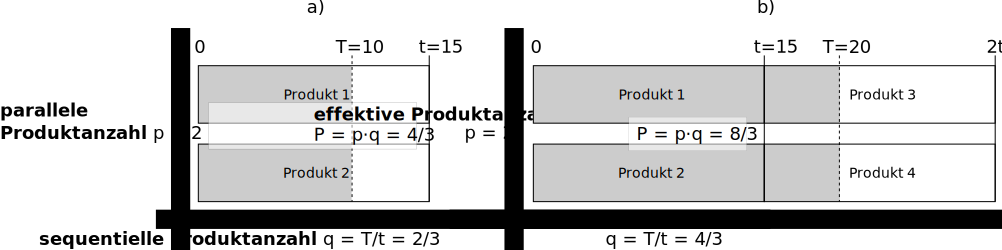
\includegraphics[width=\textwidth]{Produktanzahlen}
	\caption{Veranschaulichung des Zusammenhangs zwischen paralleler, sequentieller und effektiver Produktanzahl. In Fall a) ist der Betrachtungszeitraum $T$ kürzer als die Nutzungsdauer $t$, sodass die zwei parallel eingesetzten Produkte nur anteilig auf das Nutzungssystem angerechnet werden. In Fall b) ist der Betrachtungszeitraum länger als die Nutzungsdauer, sodass zwei Produkte voll und zwei weitere anteilig angerechnet werden.}
	\label{fig:Produktanzahlen}
\end{figure}

%Dies lässt sich mit Gleichung \ref{eq:t_tech} auch schreiben als:
%\begin{equation}
%	\label{eq:t_Fallunterscheidung}
%	t =\left\{\begin{array}{ll}  t_{\text{max}} & \mbox{falls } t_{\text{max}} < \frac{n_{\text{max}}}{h} \\ \frac{n_{\text{max}}}{h} & \mbox{sonst} \end{array}\right.
%\end{equation} \noteJ{Gleichung \ref{eq:t_Fallunterscheidung} evt. weglassen}


% b) P = N/n (Annahme: alle Produkte gleiches n)
Der zweite Ansatz zur Bestimmung der effektiven Produktanzahl basiert auf dem Verhältnis zwischen der Nutzungsmenge $n$, die ein einzelnes Produkt während seiner Nutzungsdauer abgibt und der Gesamtnutzungsmenge $N$ des Produktnutzungssystems. Unter der Annahme, dass alle konkret eingesetzten Produkte über die gleiche Nutzungsmenge verfügen, bestimmt sich die effektive Produktanzahl folgendermaßen:
\begin{equation}
	P = \frac{N}{n}
\end{equation}

Wir fassen die wichtigsten Ergebnisse dieses Abschnitts als Grundmodell zusammen: \\
\begin{mdframed}[frametitle={Grundmodell}, frametitlerule=true]
	Modellgleichung:
	\begin{equation}
		\label{eq:Grundmodell_MIPS}
		\text{MIPS} = \frac{I}{S}
	\end{equation}
	weitere Grundgleichungen:
	\begin{align}
		I &= I_P + I_N + I_W + I_R + I_\Theta + I_\text{Rest} \\[10pt]
		&= P \cdot i_P + N \cdot i_N + W \cdot i_W + R \cdot i_R + \Theta \cdot i_\Theta + I_\text{Rest}
	\end{align} \\[-35pt]
	\begin{minipage}[t]{0.49\textwidth}
		\begin{align}
			S 	&= S_D \\[10pt]
				&= N \cdot A \\[9pt]
			  n &= h \cdot t
		\end{align}
	\end{minipage}
	\begin{minipage}[t]{0.49\textwidth}
		\begin{align}
			t &= \text{min} \{t_\text{max}, t_\text{tech} := \frac{n_\text{max}}{h}\} \\
			P &= p \cdot q = p \cdot \frac{T}{t} \\
			&= \frac{N}{n}
		\end{align}
	\end{minipage}
\end{mdframed}

\end{document}